\section{Decentralized Finance (DeFi)}
\subsection{Key Features}
\begin{itemize}
  \item Currency either carries intrinsic value or created by a centralized entity.
  \begin{itemize}
    \item Government is backing the financial value of a currency (regulated, trusted)
  \end{itemize} 
  \item Blockchain's (BC) key innovations is the transfer and trade of financial assets without trusted intermediaries.
  \item Decentralized Finance (DeFi) specializes in advancing financial technologies and services on top of smart contract enabled ledgers.
\end{itemize}

\subsection{DeFi vs CeFi}
\begin{enumerate}
  \item Transparency
  \begin{itemize}
    \item Public rules and protocols.
    \item Avoid private agreements, back-deals and centralization.
  \end{itemize}
  \item Control
  \begin{itemize}
    \item DeFi gives control to its users. No-one should censor, move or destroy the users assets.
  \end{itemize}
  \item Accessibility
  \begin{itemize}
    \item Anyone with a computer, internet connection and know-how can use or create DeFi products.
  \end{itemize}
\end{enumerate}

\subsection{Properties}
\begin{enumerate}
  \item Public Verifiability
  \begin{itemize}
    \item While the DeFi app may not be fully open-sourced, the execution and bytecode must be publicly verifiable on a BC
  \end{itemize}
  \item Custody
  \begin{itemize}
    \item DeFi allows its users to control their assets at any time (no need to wait for the bank to open). Technical risks are with the user, with CeFi, is mostly with the bank (USP)
  \end{itemize}
  \item Privacy
  \begin{itemize}
    \item DeFi is present on non-privacy preserving smart contract blockchains (e.g., not on Monero).
    \item BCs offer pseudoanonymity, but no real anonymity.
    \item Centralized exchanges with KYC/AML practices are often the only viable route to convert between fiat and cryptocurrency assets.
  \end{itemize}
  \item Atomicity
  \begin{itemize}
    \item A BC transaction supports sequential actions, which can combine multiple financial operations.
    \item Flash loan example.
    \item This combination can be enforced to be atomic.
    \item While this programmable atomicity property mostly absent from CeFi, (likely costly and slow) legal agreements could enforce atomicity in CeFi as well.
  \end{itemize}
  \item Execution Order Malleability
  \begin{itemize}
    \item Users on permissionless blockchains typically share publicly the transactions.
    \item No centralized entity ordering transaction execution, peers can perform transaction fee bidding contests to steer the transaction execution order.
    \item In CeFi: regulatory bodies impose strict rules on financial institutions and services as in how transaction ordering must be enforced.
  \end{itemize}
  \item Transaction Costs
  \begin{itemize}
    \item Transaction fees in DeFi and blockchains in general are essential for the prevention of spam.
    \item In CeFi, financial institutions can opt to offer transaction services at no cost (or are mandated by governments to offer certain services for free) because of the ability to rely on KYC/AML verifications of their clients.
  \end{itemize}
  \item Anonymous Development and Deployment
  \begin{itemize}
    \item Many DeFi projects are developed and maintained by anonymous teams.
  \end{itemize}
  \item Non-stop Market Hours
  \begin{itemize}
    \item It is rare for CeFi markets to operate without downtime.
    \item DeFi has no pre- or post-market trading.
    \item System outages at CeFi stock happened.
  \end{itemize}
\end{enumerate}

\subsection{Regulation}
\begin{itemize}
  \item Regulatory uncertainty
  \item Censoring (Temporarily) Transactions
  \begin{itemize}
    \item Miners can decide to temporarily censor transactions
    \item Nodes in lightning may simply refuse a transaction (forcing the user to fall-back to on-chain payment channels).
  \end{itemize}
  \item Blacklists, Fungibility and Destruction of Assets
  \begin{itemize}
    \item Once a service provider is KYC/AML regulated, the freezing and confiscation of financial assets may be requested.
  \end{itemize}
\end{itemize}

\subsection{Future?}
DeFi could become the underlying infrastructure of future banks, whereas traditional finance / custody adapt.

\subsection{Exchange Rate}

\subsubsection{Cefi}
ask/bid, sell/buy, the last trade.
\begin{itemize}
  \item Price changes if trade happens, ask was same or lower than bid. Ask/bid submitted by users
  \item Slippage: you see a price, submit, and until its executed, price can change.
  \item Order/time important → frontrunning, more data stored on chain
\end{itemize}

\subsubsection{Defi}
ratio of pairs: function that define price.
Also slippage. 
Large swap can change price (as with CEX).

\subsection{Decentralized Swaps}
Uniswap uses X * Y = k, where k is constant, X and Y are asset values.
(if you take out X you need to provide Y).
Therefore pool can not be drained:\\
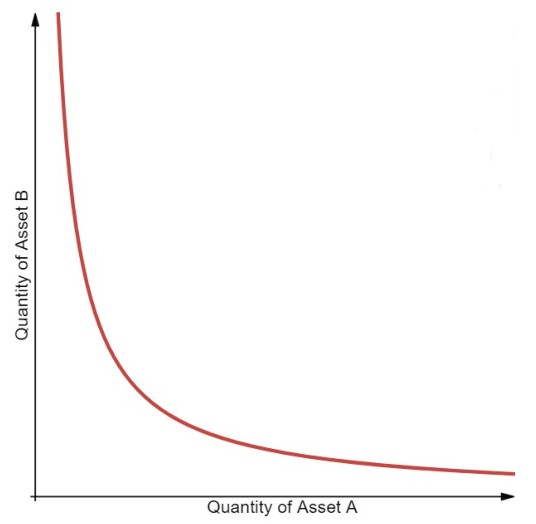
\includegraphics[width=\linewidth]{pool.jpg}

\subsubsection{Uniswap Example}
Simple exchange price calculation (Uniswap):\\
Swap for 0.5 ETH, if you send 0.5 ETH to pool:
$$200 / 1.5 \rightarrow 133 DAI \rightarrow 133 DAI for 1.5 ETH$$
Deduct 66 DAI from pool $\rightarrow$ 133/1.5 $\rightarrow$ 88 DAI for 1 ETH.
Not draining the pool, but trading with better price than resulting pool.